\chapter{Optimal coordinated control of wind farms: problem formulation and optimization methodology}\label{ch:opt_formulation}

The current chapter discusses the approach to formulating and solving the optimal coordinated wind-farm control that is the subject of the remainder of this dissertation. As introduced in Chapter~\ref{ch:introduction}, we aim to utilize individual turbines as dynamic flow actuators with the aim to optimally influence the ABL flow for increased aggregate power extraction. To this end, we use  LES, as we aim to harness turbulent flow features in the optimization process. As present-day computational resources are the decisive limiting factor in the current study, it is crucial that the employed algorithms are as efficient as possible. Therefore, we will justify methodological choices presented in this chapter through numerical examples of typical optimal control cases. 

Section~\ref{sec:problem_receding} discusses the receding horizon control approach, subdividing the time horizon into a set of discrete time windows over which power extraction is optimized. Subsequently, Section~\ref{sec:problem_formulation} introduces the mathematical formulation of the optimization problem to be solved within each time window. Thereafter, Section~\ref{sec:problem_optimization} elaborates on the gradient-based methods used to solve these optimization problems, and provides a comparison between the classically used nonlinear conjugate gradient method and the quasi-Newton L--BFGS--B method used in the current study. Next, Section~\ref{sec:problem_gradient} presents the continuous adjoint approach to numerical evaluation of the gradient required by the former algorithms, and performs a verification of the chosen approach using a representative test case. Finally, Section~\ref{sec:opt_prob_summ} summarizes the current chapter.

Parts of the contents of this chapter have been published in \cite{munters2017optimal}, ``An optimal control framework for dynamic induction control of wind farms and their interaction with the atmospheric boundary layer'', \emph{Phil. Trans. R. Soc. A} \textbf{375}, 20160100. 

\section{Receding-horizon optimization}\label{sec:problem_receding}
In a conventional optimal-control approach (see Figure~\ref{fig:block_diag}a), the system (the wind farm) is controlled by a controller that optimizes the controls ($\boldsymbol{\varphi}$) in a state model that represents the system. Usually, a receding horizon approach is used (see, e.g., Figure~\ref{fig:drawing_receding_horizon}), in which the controls are optimized for a future time window $[t,t+T]$, after which the obtained optimum ($\boldsymbol{\varphi}^{\bullet}$) is used during a control time step $T_A$. In addition, the model state is regularly adapted based on measurements in the system, minimizing the errors between the state model and the real system. The challenge for wind farms is that the detailed turbulent flow state in the atmospheric boundary layer is very high dimensional, and an accurate state model (e.g. based on large-eddy simulations) is computationally very expensive, so that it is impossible to implement in a real-time controller. Therefore, wind-farm control in practice requires extensive simplifying assumptions that may limit \emph{a priori} the performance of the controller. Because of this, the development of practical cooperative wind-farm controllers remains an open issue to date, in particular for the case of power maximization through mitigation of unfavorable wake interactions.

Throughout the current work, the same approach to wind-farm control is followed as introduced in \cite{goit2015optimal}. Instead of focusing on the direct formulation of a real wind-farm controller for increased energy extraction, optimal controls are pursued in a very accurate state representation of the wind-farm boundary layer, i.e. based on LES, that resolves the large turbulent flow structures in the atmospheric boundary layer and their interaction with the wind turbines both in space and in time (see Figure~\ref{fig:block_diag}b). Furthermore, the state estimation is dropped: the full spatio-temporal wind-farm flow field is available to the optimizer. Such an approach is unfeasible for real control, as LES is to date still too computationally expensive for real-time control, and full flow-field information is impossible. However, it allows for exploring the potential of improved energy extraction by wind-farm control, and may help in identifying new ways in which large wind farms can optimally interact with the atmospheric boundary layer. As will be discussed in further chapters, the work performed in the context of this dissertation has contributed to novel and optimal control studies, but also provided first steps towards an increased understanding of the mechanisms that could lead to practical controller implementation.

\begin{figure}
	\centering
	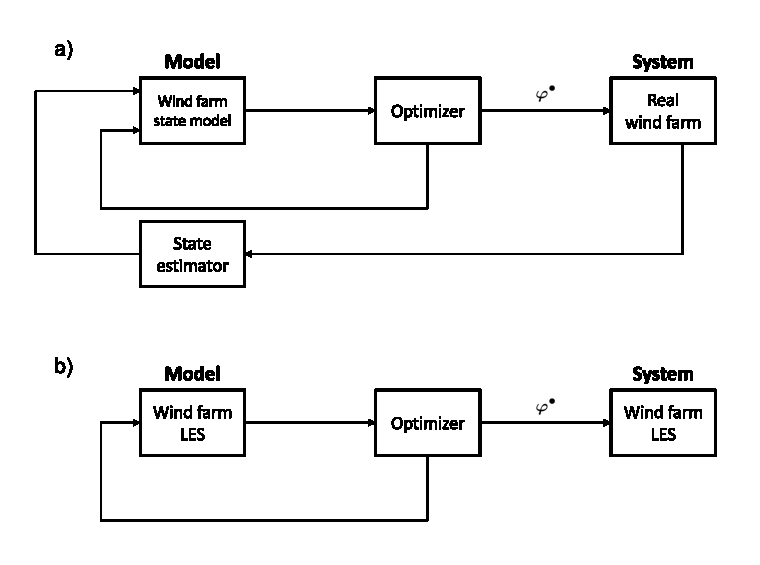
\includegraphics[width=0.7\textwidth]{chapters/optimal_control_problem/figure1.eps}
	\caption[Model-predictive control approach applied to wind farms. Conventional MPC \& Benchmark optimal control framework applied in the current study.]{Model-predictive control applied to wind farms. a) Conventional feedback MPC of a wind farm. b) Benchmark optimal control framework of a wind farm LES considered in the current study.}\label{fig:block_diag}
\end{figure}

Similar to \cite{goit2015optimal}, we use a receding horizon optimization approach as shown in Figure~\ref{fig:drawing_receding_horizon}. Given a control time horizon $T$, controls are optimized to yield maximum energy extraction. Further details are provided in following sections. Part of the resulting optimal controls $\boldsymbol{\varphi}^{\bullet}$ are then used for a time period $T_A \leq T$, during which we advance the wind-farm LES system in time. Subsequently, control optimization over a new time horizon is initiated, and the process is repeated for each of the $N_w$ control windows in order to control wind-farm operation of the total time $T_{tot} = N_w T$. 

Note that, in a true optimal control setting, we aim to choose $T = T_{tot}$, resulting in a single control window over the full time horizon. However, $T$ is limited by the fact that classical adjoint methods fail to provide useful gradient information of chaotic systems such as turbulent flows over long time horizons. Although promising solutions to this problem based are currently under development (see, e.g. \citealp{wang2014least, chater2016simplified}), the incorporation thereof lies outside the scope of this thesis. Furthermore, $T$ is limited by disk storage and memory requirements, resulting from the fact that the backwards integration of the adjoint equations requires the full space-time state of the forward flow solution (see Equation \ref{eq:adjoint_momentum} further below). In the current manuscript, we take $T$ as long as possible, while satisfying the constraints mentioned in this paragraph. Also, due to the non-convex nature of the optimization problems considered in this thesis, even upon full convergence of the algorithm, the gradient-based optimization will most likely result in a local optimum instead of the true global optimal control solution of the problem. Nonetheless, the terminology `optimal control' will continue to be used for the optimizations throughout this thesis. 

\begin{figure}[]
	\centering
	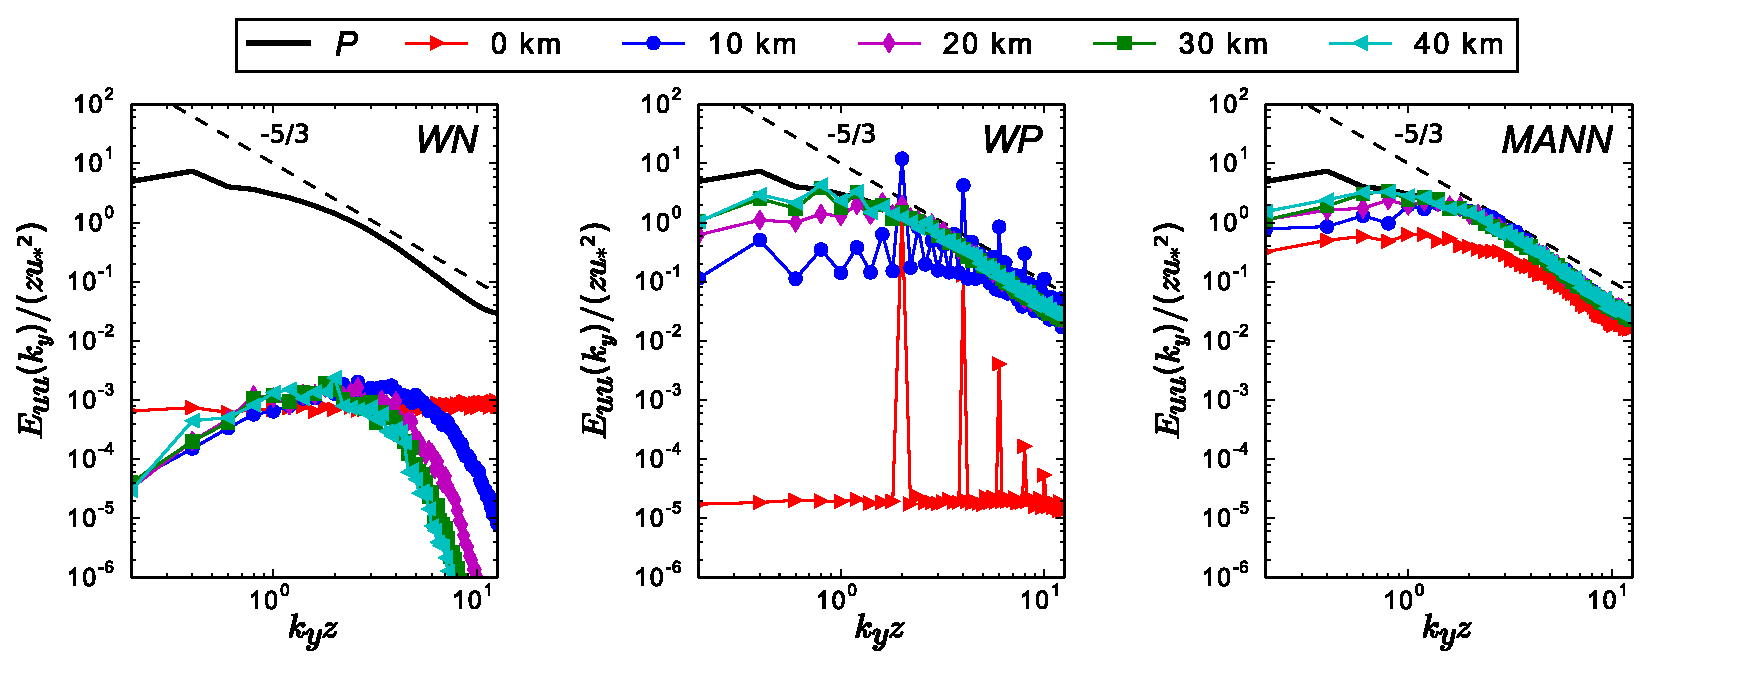
\includegraphics[width=0.65\linewidth]{chapters/optimal_control_problem/figure2.eps}
	\caption[Receding horizon optimization framework for optimal control of wind farms.]{Receding horizon optimization framework for optimal control of wind farms. Figure adapted from \cite{goit2015optimal}.}
	\label{fig:drawing_receding_horizon}
\end{figure}

The flow advancement time $T_A$ is chosen based on a trade-off between limiting overall computational expenses, favoring $T_A/T \rightarrow 1$, and averting finite-horizon optimization effects, favoring $T_A/T \rightarrow 0$. Figure~\ref{fig:T_A} qualitatively illustrates the influence of $T_A$ on the temporal smoothness of the wind farm power extraction for an optimal induction control case (case C3t0 from Chapter~\ref{ch:opt_induction}, further details omitted here). The figure shows the normalized power extraction for $T_A = T/2 = 120$ s (top) and $T_A = T/4 = 60$ s (bottom) respectively, where both simulations apply an equal prediction horizon $T = 240$ s. For $T_A = T/2$ it can be seen in Figure~\ref{fig:T_A} that, within each window, power extraction is initially reduced. This causes flow conditions that lead to an increased power extraction later in the window. By stringing the windows together, a sawtooth-like behavior of power extraction is created. Reducing $T_A$ diminishes this effect, as shown in Figure~\ref{fig:T_A}b, but leads to a doubling in computational cost for a given total time $T_{tot}$. Although present-day computational resources have limited us to using $T_A = T/2 = 240$ s for the cases presented in this dissertation, we advise to reduce $T_A/T$ in the future to obtain reduced ramps in power production and mitigate finite-horizon effects.

\begin{figure}
	\centering
	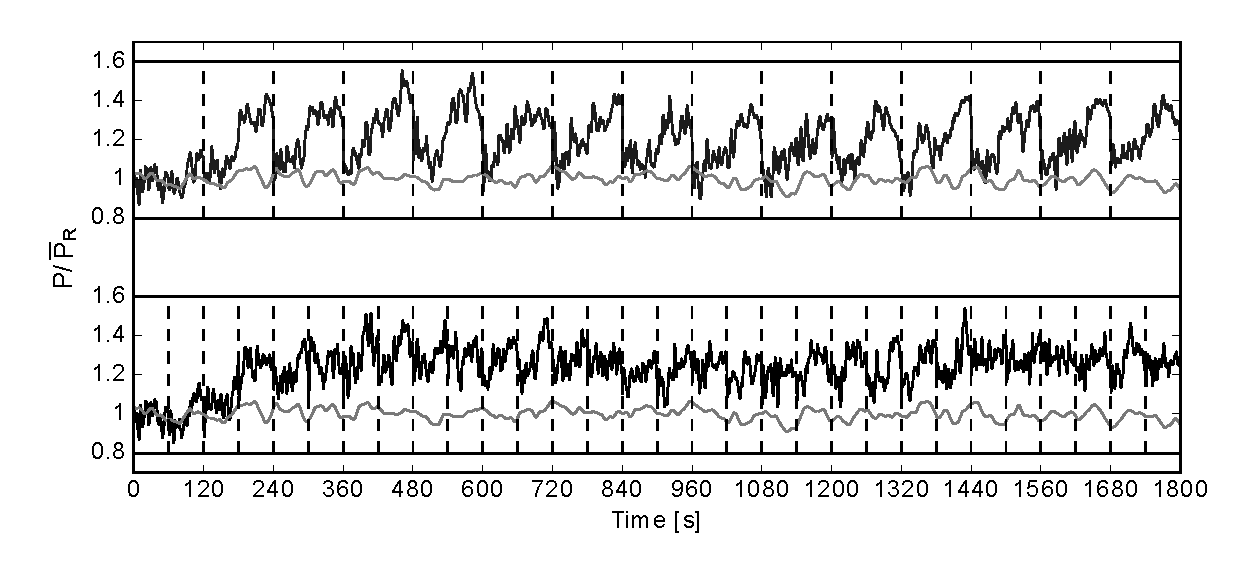
\includegraphics[width=\linewidth]{chapters/optimal_control_problem/figure10.eps}
	\caption[Dynamic behavior of optimized power extraction for case C3t0 from Chapter~\ref{ch:opt_induction}, normalized by a greedy control reference case.]{Dynamic behavior of optimized power extraction for case C3t0 from Chapter~\ref{ch:opt_induction}, normalized by a greedy control reference case (shown in gray). \emph{Top: } $T_A = T/2 = 120$ s. \emph{Bottom: } $T_A = T/4 = 60$ s. The dashed vertical lines indicate the flow advancement windows.\label{fig:T_A}}
\end{figure}


\section{Optimal control problem formulation}\label{sec:problem_formulation}

In this section, the optimal control problem, which is solved in every window of the aforementioned receding-horizon method, is mathematically formulated. Firstly the objective, or \emph{cost} functional, defined. Thereafter, the wind turbine controls are briefly revised. Finally, the PDE-constrained optimization problem that is used throughout the remainder of this work is defined. 

\subsubsection{Cost functional}
The aim of the optimal control is translated into the minimization of a scalar cost functional $\J$. In all optimal control cases throughout this thesis, this cost functional is defined as the negative of the aggregated energy extracted from the ABL by the wind farm (opposite due to minimization convention), i.e.
\begin{equation}\label{eq:costfunction}
	\J = - \Tint \sum_{i=1}^{N_t} P_i(t) \dt = - \Tint \sum_{i=1}^{N_t} \frac{1}{2} a \ctihat V_i^3 A_i \dt,
\end{equation}
with the turbine area $A_i$, time-filtered thrust coefficient $\widehat{C}_T'$, scaling parameter $a = C_P'/\widehat{C}_T'$, and disk-averaged axial velocity $V_i = (1/A_i) \sint  \R(\bs{x}) \ufilt \cdot \eperp \dx$, as defined in Section~\ref{sec:meth_adm}. Note that there is no cost associated with control actions, and no considerations on turbine loading are taken: wind-farm power is optimized at all cost throughout this thesis. 

\subsubsection{Wind turbine controls}\label{sec:opt_problem_controls}
The individual wind turbines are controlled dynamically in such a way as to actively influence the turbulent ABL flow to yield favorable conditions for farm-aggregated power extraction. In the non-rotating actuator disk models considered in this thesis, this influence consists solely of the thrust force enacted upon the flow. Recall from Section~\ref{sec:meth_adm} that this thrust force $\bs{f}_i$ was parametrized as
\begin{equation}\label{eq:problem_thrust}
\bs{f}_i(\bs{x}) = -\frac{1}{2} \ctihat V_i^2 A_i \R_i(\bs{x}) (\bs{e}_x \cos \theta_i + \bs{e}_y \sin \theta_i).
\end{equation} 
The control parameters for the turbine models were also introduced in Section~\ref{sec:meth_adm}, and consist of the thrust coefficient setpoint $\cti$ and yaw rate $\omega_i$ for every turbine $i = 1 \dots N_t$ in every discrete time step, with shorthand notation $\bs{\varphi}(t) = [\ctn{1}(t), \dots, \ctn{N_t}(t), \omega_1(t), \dots, \omega_{N_t}(t)] = [\bs{C}_T'(t), \bs{\omega}(t)]$. The influence of these control parameters on the thrust force in \eqref{eq:problem_thrust} is governed by their influence on the thrust coefficient $\ctihat$ and yaw angle $\theta_i$ in the following set of ODEs:
\begin{align}
\tau \ddt{\ctihat} &= \cti - \ctihat \label{eq:problem_timefilter_def},\\
\ddt{\theta_i} &= \omega_i \label{eq:problem_omega_def}.
\end{align}

%
% This influence originates from the thrust force enacted by the turbine upon the flow, characterized by its magnitude and orientation. The orientation is aligned with the rotor-perpendicular vector $\eperpi = \bs{e}_x \cos \theta_i + \bs{e}_y \sin \theta_i$, with $\theta_i$ defined as the yaw angle of the turbine, which can be controlled using the active yaw system in modern turbines. The magnitude of this force is determined by the pitch angle of the blades as well as the tip speed ratio of the turbine rotor. As discussed in Chapter~\ref{ch:methodology} however, we don't resolve the effects of these parameters, but lump them into a (time-filtered) single axial thrust coefficient $\widehat{C}_{T,i}'$, and parametrize the force as 
%\begin{equation}
%	\bs{f}_i(\bs{x}) = -\frac{1}{2} \ctihat V_i^2 A_i \R_i(\bs{x}) (\bs{e}_x \cos \theta_i + \bs{e}_y \sin \theta_i),
%\end{equation} 
%which is then smeared out to the LES grid using a smooth kernel representation of the turbine geometry $\R_i(\bs{x})$. For any given turbine $i$, we will hence actively control the force enacted on the flow by adapting the turbine state in the form of its thrust coefficient $\widehat{C}_{T,i}'$ and yaw angle $\theta_i$. 
%
%These parameters are not controlled directly, instead the controls consist of a dynamic thrust coefficient setpoint $C_{T,i}'(t)$ and a yaw rate $\omega_i(t)$, with shorthand notation $\bs{\varphi}(t) = [\bs{C}_T'(t),\ \bs{\omega}(t)] = [\ctn{1}(t), \dots, \ctn{N_t}(t),\ \omega_1(t), \dots, \omega_{N_t}(t)]$. These controls are related to the turbine states mentioned above as
%\begin{align}
%	\tau \ddt{\ctihat} &= \cti - \ctihat \label{eq:timefilter_def},\\
%	\ddt{\theta_i} &= \omega_i \label{eq:omega_def}.
%\end{align}
%Equation \eqref{eq:timefilter_def} is a first-order exponential time filter with a time constant $\tau$, which characterizes the turbine response time to variations in thrust setpoints (see Figure~\ref{fig:cthat_form} for an illustration of this concept). This would, for example, fit in a hierarchical approach to wind-farm control, in which wind-farm control signals are passed on to individual turbine controllers that themselves may not react instantaneously to the control signals. Moreover, increasing $\tau$ allows to assess the effect on power gains of limiting dynamics in turbine operation, which could be beneficial for turbine lifetime. To allow for realistic technical behavior of the modeled turbines, box constraints are imposed on the thrust coefficients setpoints. In addition, by controlling the yaw rate $\omega_i$ instead of directly controlling the angle $\theta_i$ in equation \eqref{eq:omega_def}, the inherent technical limitations on active yaw systems can be implemented as simple box constraints, facilitating the use of many optimization algorithms (see Section~\ref{sec:problem_optimization}).

\subsubsection{Optimal control problem}
In addition to the wind-turbine states defined through \eqref{eq:timefilter_def} -- \eqref{eq:omega_def}, the ABL states in the form of flow field variables $\ufilt$ and $\ptilde$ have to abide by the filtered Navier--Stokes equations introduced in Section~\ref{sec:meth_governing}. Defining $\bs{q}(\bs{x},t) = [\ufilt(\bs{x},t),\ \ptilde(\bs{x},t),\ \widehat{\bs{C}}_T'(t),\ \bs{\theta}(t)]$ as a shorthand notation for the state variables, the optimal wind-farm control can be formulated as a PDE-constrained optimization problem:
\begin{mini!}[1]
	{\scriptsize \bs{\varphi}, \bs{q}}{\J(\bs{\varphi}, \bs{q}) = - \Tint \sum_{i=1}^{N_t} \frac{1}{2} a \ctihat~V_i^3 A_i \dt}{\label{eq:costfunction_inside_problem}}{}
%	\addConstraint{\small \frac{\partial \utilde}{\partial t} + \big(\utilde \cdot \nabla \big)\utilde }{\small = - \nabla (\ptilde + \ptilde_\infty) / \rho - \nabla \cdot \boldsymbol{\tau}_{sgs} + \sum_{i=1}^{N_t} \bs{f}_i\ + \bs{f}_{\text{fr}} }{\small \text{in } \Omega \times (0,T] \label{eq:NSmomentum_constraint}}
	\addConstraint{\small \frac{\partial \utilde}{\partial t} + \big(\utilde \cdot \nabla \big)\utilde }{\small = - \nabla \ptilde / \rho - \nabla \cdot \boldsymbol{\tau}_{sgs} + \sum_{i=1}^{N_t} \bs{f}_i\ + \bs{f}_{\text{fr}}\ \ }{\small \text{in } \Omega \times (0,T] \label{eq:NSmomentum_constraint}}	
	\addConstraint{\small \nabla \cdot \utilde}{\small =0, \label{eq:NScontinuity_constraint}}{\small \text{in } \Omega \times (0,T]}
	\addConstraint{\small \tau \ddt{\ctihat}}{\small =\cti - \ctihat \label{eq:ctihat_constraint}}{\small i=1...N_t~\text{in } (0,T]}
	\addConstraint{\small \ddt{\theta_i}}{\small = \omega_i \label{eq:omega_constraint}}{\small i=1...N_t~\text{in } (0,T]}
	\addConstraint{\small C_{T,\text{min}}' \leq}{\small  \cti \leq C_{T,\text{max}}' \label{eq:boxct_constraint}}{\small i=1...N_t~\text{in } (0,T]}
	\addConstraint{\small -\omega_{\text{max}} \leq}{\small  \omega_i \leq \omega_{\text{max}} \label{eq:boxomega_constraint}}{\small i=1...N_t~\text{in } (0,T].}
\end{mini!}

The equality constraints on the state variables in \eqref{eq:NSmomentum_constraint} - \eqref{eq:omega_constraint} will be grouped using the shorthand notation $\bs{B}(\bs{\varphi}, \bs{q}) = 0$ throughout the current chapter. Note that evaluating these constraints requires a full LES of the filtered Navier--Stokes equations using the method discussed in Chapter~\ref{ch:methodology}. Note that, by defining the parameters $C_{T,\text{min}}'$, $C_{T,\text{max}}'$, and $\omega_{\text{max}}$ in the box constraints \eqref{eq:boxct_constraint} -- \eqref{eq:boxomega_constraint}, one can define exclusive induction control, exclusive yaw control, and combined induction-yaw control cases, as will be done in subsequent chapters. The following sections will discuss how the optimization problem is solved in the current work. 

\section{Optimization algorithms}\label{sec:problem_optimization}

The current section discusses the methodology of solving the optimization problem defined in \eqref{eq:costfunction}. Instead of solving the problem in its original formulation, i.e. by optimizing the cost functional $\J(\bs{\varphi}, \bs{q})$ over both the control and state space given all constraints, the problem is solved in a reduced formulation as is common practice in PDE-constrained optimization \citep{borzinschulz}. In the reduced formulation of the optimization problem, the dependency of the state variables on the control parameters, denoted as $\bs{q}(\bs{\varphi})$, is explicitly satisfied throughout the optimization process, therefore leaving a reduced problem to be optimized over the control space only. The only remaining constraints are the original box constraints on the controls, i.e. 

\begin{mini!}|s|
	{\bs{\varphi}}{\Jtilde(\bs{\varphi}) \equiv \J(\bs{\varphi},\bs{q}(\bs{\varphi}))}{ \label{eq:optimizationproblem_reduced}}{}
	\addConstraint{\bs{\varphi}_{\text{min}} \leq\ }{ \bs{\varphi} \leq\  \bs{\varphi}_{\text{max}}.\quad \label{eq:box_constraint_reduced}}{}
\end{mini!}

Given the high computational cost of evaluating the reduced cost functional, i.e. by LES of the filtered Navier--Stokes equations, the constrained optimization problem in \eqref{eq:optimizationproblem_reduced} is solved using a suitable gradient-based method. The evaluation of the cost functional gradient with respect to the control parameters is performed using the continuous adjoint method, which involves simulation of an auxiliary set of PDEs at a cost equivalent to the standard LES. The gradient evaluation procedure is further detailed below in Section~\ref{sec:problem_gradient}. 

The remainder of the current section discusses the quasi-Newton L--BFGS--B optimization algorithm used throughout this thesis, and compares it to a non-linear conjugate gradient (CG) method that was used in earlier adjoint gradient-based control studies of turbulent flows \citep{bewley2001dns, goit2015optimal,goit2016optimal}. Both algorithms are line-search methods, in which the controls $\bs{\varphi}$ are updated iteratively as 
\begin{equation}
	\blds{\varphi}_{k+1} = \blds{\varphi}_k + \alpha_k \blds{d}_k,
\end{equation}
where $k$ denotes the iteration index, $\bs{d}_k$ is the current search direction, and $\alpha_k$ is a suitable step length resulting from a line search. The CG and L--BFGS--B algorithms below differ mainly in the way $\bs{d}_k$ and $\alpha_k$ are selected.

	\subsection{Non-linear Conjugate Gradient method}\label{sec:problem_cg}
	The non-linear CG method has been the method of choice for DNS- or LES-constrained optimization of turbulent flows since the advent of the methodology \cite{collis2000large, bewley2001dns}. The main approach behind CG methods is to produce subsequent conjugate search directions as
	\begin{equation}
		\bs{d}_k = -\nabla \Jtilde + \beta_k \bs{d}_{k-1}.
	\end{equation}
	Different non-linear CG methods exist based on the definition of the scalar parameter $\beta_k$. In the context of PDE-constrained optimization of turbulent flows, the Polak--Ribi\`ere variant has been successfully used in the past, in which $\beta_k$ is calculated as 
	\begin{equation}
		\beta_k = \frac{ \big( \nabla \Jtilde_k - \nabla \Jtilde_{k-1} \big)^T  \nabla \Jtilde_k}{\big(\nabla \Jtilde_{k-1}\big)^T  \nabla \Jtilde_{k-1}}.
	\end{equation}
	
	Further, following earlier optimization studies with unsteady turbulence-resolving flow models \citep{bewley2001dns, delport2009constrained, goit2015optimal}, the step length $\alpha_k$ is determined based on the gradient-free Brent exact line-search algorithm, which solves the following one-dimensional optimization problem by iteratively reducing an interval which is guaranteed to contain the optimal steplength $\alpha$:
	\begin{equation}
		\alpha_k = \argmin_\alpha{\Jtilde}(\blds{\varphi}_k + \alpha \blds{d}_k).\label{eq:linesearch_exact}
	\end{equation}
	In practice, this line search is terminated after a fixed amount of iterations. Details on the implementation in OSP-Wind can be found in \cite{delport2009constrained}. The box constraints in \eqref{eq:box_constraint_reduced} are respected by projecting the step direction on the feasible set.
	
	Assuming that $\Jtilde_k = \Jtilde(\bs{\varphi}_k) \equiv \Jtilde(\bs{\varphi}_{k-1} + \alpha_{k-1} \bs{d}_{k-1})$ is known at the start of iteration $k$ from the line search in iteration $k-1$, within each iteration the gradient $\nabla \Jtilde_k = \nabla \Jtilde (\bs{\varphi}_k)$ is to be calculated only once to determine the step direction $\bs{d}_k$. Subsequently, each subiteration of the line-search algorithm requires one additional functional evaluation $\Jtilde(\bs{\varphi}_k + \alpha \bs{d}_k)$.

	\subsection{Limited-memory BFGS method with Bounds support\\(L--BFGS--B)}
	It has been shown for turbulent flow optimization that the inclusion of curvature information as in quasi-Newton methods can lead to a significant computational cost reduction in terms of functional and gradient evaluations \citep{nita2016efficiency}. The limited-memory BFGS method with bounds support (L--BFGS--B) algorithm developed by \cite{byrd1995limited} is a widely used quasi-Newton method, suitable for the constrained optimization problem at hand. 
	
	At the beginning of each iteration, a quadratic model of the cost functional is constructed based on the current iterate $(\blds{\varphi}_k, \Jtilde_k)$, the current gradient $\nabla \Jtilde_k$, and a positive definite limited-memory BFGS Hessian approximation $B_k$. The latter approximation is constructed from information retained from previous iterations through a set of $m$ correction pairs $\{(\blds{\varphi}_{i+1}- \blds{\varphi}_i), (\nabla \Jtilde_{i+1} - \nabla \Jtilde_i)\}$, for $i = k-1, \dots, k-m$ \citep{liu1989limited}. The quadratic model is then minimized while respecting the bound constraints resulting in an intermediate control $\overline{\bs{\varphi}}_{k+1}$ as 
	\begin{align}
	\overline{\bs{\varphi}}_{k+1} = &\argmin_{\bs{\varphi}}{\Jtilde_k + \big(\nabla \Jtilde_k\big)^T (\blds{\varphi} - \blds{\varphi}_k) + \frac{1}{2} (\blds{\varphi} - \blds{\varphi}_k)^T B_k (\blds{\varphi} - \blds{\varphi}_k)}. \nonumber\\
		&{\rm s.t.} \qquad \qquad \qquad \bs{\varphi}_{\rm min} \leq \bs{\varphi} \leq \bs{\varphi}_{\rm max}
	\end{align}
	Subsequently, the step direction is oriented towards this optimizer of the quadratic model as
	\begin{equation}
		\bs{d}_k = \overline{\bs{\varphi}}_{k+1} - \bs{\varphi}_k. 
	\end{equation}
	The step length $\alpha_k$ is determined by an inexact Mor\'e -- Thuente line-search algorithm \citep{more1994line}. Instead of solving a one-dimensional optimization problem as in \eqref{eq:linesearch_exact}, the line search is terminated once a suitable step length $\alpha$ is found such that the strong Wolfe conditions are satisfied \citep{wolfe1969convergence, wolfe1971convergence}:
	\begin{align}
		\Jtilde(\bs{\varphi}_k + \alpha_k \bs{d}_k) &\leq \Jtilde_k + c_1 \alpha_k \big( \nabla \Jtilde_k \big)^T \bs{d}_k, \\
		\vert \big( \nabla\Jtilde(\bs{\varphi}_k + \alpha_k \bs{d}_k) \big)^T \bs{d}_k \vert &\geq c_2 \vert \big( \nabla \Jtilde_k \big)^T \bs{d}_k \vert.
	\end{align}
	These conditions are also known as the \emph{sufficient decrease} (or \emph{Armijo}) condition and the \emph{curvature} condition respectively. The scaling parameters in these conditions are typically chosen as $c_1 = 10^{-4}$ and $c_2 = 0.9$. Note that the algorithm already provides an estimation for a suitable step length, i.e. a unit step $\alpha_k = 1$. This is used to initialize the line search, as is standard practice for quasi-Newton methods \citep{wright1999numerical}. It will be shown that, for the wind-farm control cases in this thesis, the unit step often already satisfies the Wolfe conditions, and no further line search is required.
	
	At the start of optimization iteration $k$, both the cost functional $\Jtilde_k$ and its gradient $\Jgrad_k$  are known from evaluating the Wolfe conditions in the previous iteration. Determining the step direction by constructing and optimizing the quadratic model requires no further functional evaluations. Subsequently, evaluating the Wolfe conditions for the unit step length with $\bs{\varphi}_{k+1} = \overline{\bs{\varphi}}_{k+1}$ requires one functional and one gradient evaluation. If the Wolfe conditions are not met, each subsequent line-search iteration requires one additional combined functional and gradient evaluation. 
	
	\subsection{Performance comparison}\label{sec:problem_performance}
	Given the high cost of evaluating both the cost functional and its gradient, i.e. by simulation of the (adjoint) Navier--Stokes PDEs, it is of primordial importance to select an algorithm with most favorable convergence properties in terms of PDE evaluations.
	
	Figure~\ref{fig:cg_bfgs} presents the cost function decrease for an optimization window of the C3t0 case from Chapter~\ref{ch:opt_induction} (computational setup not further detailed here) as a function of PDE evaluation for the Polak--Ribi\`ere non-linear CG method and the L--BFGS--B method elaborated above. The figure illustrates that the use of additional knowledge of curvature information employed by the L--BFGS--B algorithm significantly speeds up convergence compared to CG. Earlier, similar behavior was also shown for a low-Reynolds-number turbulent channel flow case \citep{nita2016efficiency}. Since the amount of PDE evaluations is the main driver behind the computational cost of the optimal control simulations, it can be seen that, for a given decrease in the cost functional, computational efforts are reduced by a factor 4 for L--BFGS--B compared to CG. The main reason behind this behavior is that, for the current problem, the CG method wastes a lot of PDE evaluations in the Brent line search that do not result in cost functional improvements (indicated by the horizontal plateaus in Figure~\ref{fig:cg_bfgs}), whereas the L--BFGS--B method mostly takes full Newton steps without any further required line search. The performance comparison presented in this section justifies the use of L--BFGS--B throughout the remainder of this text. 
	
	\begin{figure}
		\centering
		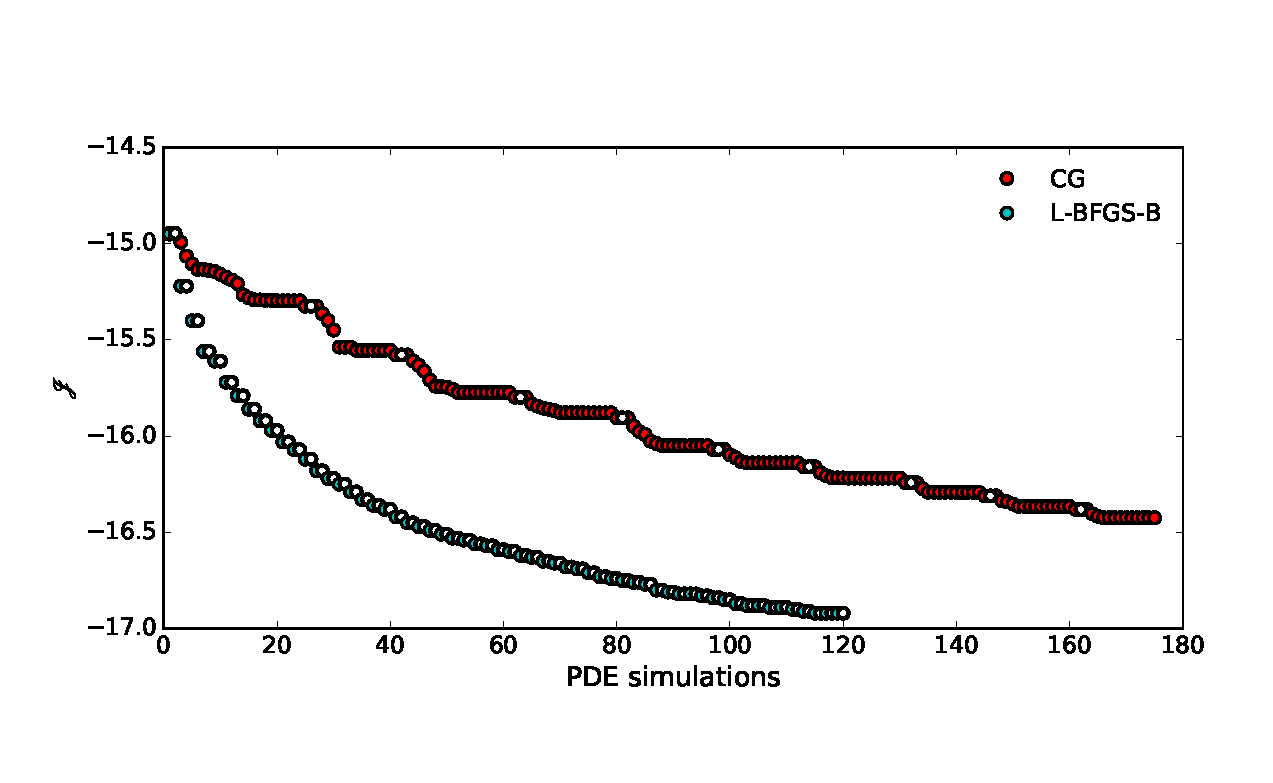
\includegraphics[width=\linewidth]{chapters/optimal_control_problem/figure5.eps}
		\caption[Cost functional decrease as a function of PDE simulations for a non-linear CG and L--BFGS--B algorithm applied to a typical wind-farm optimization window.]{Cost functional decrease as a function of PDE simulations for a non-linear CG and L--BFGS--B algorithm applied to a typical wind-farm optimization window. \emph{Filled circles: } LES, \emph{Open circles: } adjoint. }
		\label{fig:cg_bfgs}
	\end{figure}
	
	
\section{Gradient evaluation of the reduced cost functional}\label{sec:problem_gradient}
	Here, we discuss how the gradient of the reduced cost functional with respect to the control variables $\bs{\varphi}$ is evaluated. Firstly, some definitions are given and the necessity of an efficient gradient evaluation is shown. Thereafter, the continuous adjoint method is introduced, resulting in the adjoint Navier--Stokes equations and the adjoint gradient expression. Finally, the adjoint gradient is verified in a comparative study with a finite difference approximation of the reduced functional gradient. 

	We interpret the gradient of the reduced cost functional, denoted as $\nabla \Jtilde$,  as the Riesz representation of the G\^ateaux derivative operator at $\bs{\varphi}$ in any arbitrary direction $\delta \bs{\varphi}$ (see, e.g. \cite{troltzsch}):
	\begin{equation}
		\Jtilde_{\bs{\varphi}}(\delta \bs{\varphi}) \equiv \lim_{t\downarrow0} \frac{\Jtilde(\bs{\varphi}+t\ \delta \bs{\varphi}) - \Jtilde(\bs{\varphi})}{t} = (\nabla \Jtilde, \delta \bs{\varphi}) \qquad \forall \ \delta \bs{\varphi} \in  U,\label{eq:gateauxder}
	\end{equation}
	with $U$ the control Hilbert space. In the above equation, and in the remainder of this chapter, we define inner products between two variables $\bs{a}$ and $\bs{b}$ as 
	\begin{equation*}
		(\bs{a}, \bs{b}) = \stint \bs{a} \cdot \bs{b}\ \dx\ \dt, \qquad \text{or} \qquad 
		(\bs{a}, \bs{b}) = \Tint \bs{a} \cdot \bs{b}\ \dt,
	\end{equation*}
	depending on the respective spaces in which they are defined. The multiplicative operator $\cdot$ can be interpreted as a regular scalar multiplication or a dot product depending on the dimensionality of $\bs{a}$ and $\bs{b}$.

	Through the definition of the reduced cost functional $\Jtilde(\bs{\varphi}) \equiv \J(\bs{\varphi}, \bs{q}(\bs{\varphi}))$, and by applying the chain rule, the gradient can be further expressed as 
	\begin{equation}
		\innerproduct{\nabla \Jtilde}{\delta \bs{\varphi}} = \innerproduct{\pder{\Jtilde}{\bs{\varphi}}}{\delta \bs{\varphi}} + \innerproduct{\pder{\Jtilde}{\bs{q}}}{\delta \bs{q}},
	\end{equation}
	with $\delta \bs{q} \equiv ( \partial \bs{q}/ \partial \bs{\varphi})\delta \bs{\varphi}$ the variation in state variables incurred through the control variation, governed by the state equations $\bs{B}(\bs{\varphi}, \bs{q}) = 0$. 
	Evaluating this term is computationally prohibitive for virtually all relevant practical applications, as this requires solving the state equations for each possible dimension in $\bs{\varphi}$. For example, for the wind-farm application considered here, the (discretized) control space has a dimensionality in the order of $10^4 - 10^5$, and straightforward evaluation would require this many PDE simulations. 

	In contrast, the adjoint method allows to reformulate the problem such that $\delta \bs{q}$ need not be explicitly evaluated, at the cost of solving an additional set of adjoint PDEs per dimension in $\J$, independently of the dimensionality of the control space $U$. Given that a multitude of problems involve interest in  only low-dimensional performance indicators, such as  the scalar aggregated wind-farm power in the current case, this fact explains the wide-spread use of adjoint methods in PDE-constrained optimization problems for various applications (see, e.g. \cite{choi1999instantaneous, aage2008topology, dekeyser2014divertor})
	
	The remainder of the current section focuses on the conceptual derivation of the adjoint equations associated with the given optimal control problem. Although the concrete elaboration of this derivation is relatively straightforward, it is also lengthy. For case of readability and brevity, we focus here on the concept, and discuss the concrete derivation of non-standard terms that are original contributions of the author in Appendix~\ref{ch:app_adj_der}.

	\subsection{Continuous adjoint method}
	In the current dissertation, the continuous adjoint method is used to circumvent the explicit evaluation of the state variation $\delta \bs{q}$ incurred by control variations when evaluating the cost functional gradient $\nabla \Jtilde$ defined in the previous section. The formal Lagrangian approach \citep{troltzsch, borzinschulz} allows to derive the adjoint equations by postulating vanishing gradients of the Lagrangian function with respect to the state variables $\bs{q}$. The following explanation largely follows the derivation from \cite{goit2015optimal}, Appendix C. The Lagrangian is constructed by adding the state constraints $\bs{B}(\bs{\varphi}, \bs{q})$ to the cost functional through the use of Lagrange multipliers, or \emph{adjoint} variables, $\bs{q}^*$:
	\begin{equation}
		\Lagr(\bs{\varphi}, \bs{q}, \bs{q}^*) = \J(\bs{\varphi}, \bs{q}) + \innerproduct{\bs{q}^*}{\bs{B}(\bs{\varphi}, \bs{q})}
	\end{equation} 
	Using the implicit relation $\bs{q}(\bs{\varphi})$ used in the reduced formulation of the problem 
	\eqref{eq:optimizationproblem_reduced}, which is equivalent to $\bs{B}(\bs{\varphi}, \bs{q}(\bs{\varphi})) \equiv 0$, it can be seen that
	\begin{align}
	\Jtilde(\bs{\varphi}) &\equiv  \J(\bs{\varphi}, \bs{q}(\bs{\varphi})) \nonumber\\ 
						  & = \J(\bs{\varphi}, \bs{q}(\bs{\varphi})) + \innerproduct{\bs{q}^*}{\bs{B}(\bs{\varphi}, \bs{q}(\bs{\varphi}))} =\Lagr(\bs{\varphi}, \bs{q}(\bs{\varphi}), \bs{q}^*). \label{eq:jtilde_lagr}
	\end{align} 
	Further, the state equations $\bs{B}(\bs{\varphi}, \bs{q}) = 0$ are linearized around a base solution $(\bs{\varphi}, \bs{q})$ in a direction $(\delta \bs{\varphi}, \delta \bs{q})$ as
	\begin{equation}
		\pder{\bs{B}}{\bs{\varphi}} \delta \bs{\varphi} + \pder{\bs{B}}{\bs{q}} \delta \bs{q} = 0, 
	\end{equation}
	which defines the linear operators $\partial \bs{B} /\partial \bs{\varphi}$ and $\partial \bs{B} /\partial \bs{q}$. The adjoint identity is used to define the adjoint linear operator $\big[ \partial \bs{B} /\partial \bs{q}\big]^*$ associated with $\partial \bs{B} /\partial \bs{q}$ as
	\begin{equation}
		\innerproduct{\bs{q}^* }{\pder{\bs{B}}{\bs{q}} \delta \bs{q}} \equiv \innerproduct{\bigg[     \pder{\bs{B}}{\bs{q}}\bigg]^* \bs{q}^* }{ \delta \bs{q} } + BT,  \label{eq:adjoint_identity}
	\end{equation}
	and similarly for $\partial \bs{B} /\partial \bs{\varphi}$. These adjoint operators are typically found by transferring differential operators from one variable to the other through integration by parts, and $BT$ represent the boundary terms that originate during this procedure. Combining \eqref{eq:jtilde_lagr} and \eqref{eq:adjoint_identity}, the gradient of the reduced cost functional can be reformulated as	
	
	{\small
	\begin{align}
		\innerproduct{\nabla \Jtilde}{\delta \bs{\varphi}} &= \innerproduct{\pder{\J}{\bs{\varphi}}}{\delta \bs{\varphi}} + \innerproduct{\bs{q}^*}{\pder{\bs{B}}{\bs{\varphi}}\delta \bs{\varphi}} + \innerproduct{\pder{\J}{\bs{q}}}{\delta \bs{q}} + \innerproduct{\bs{q}^*}{\pder{\bs{B}}{\bs{q}}  \delta \bs{q}  } \nonumber \\
		&= \innerproduct{\bigg\{ \pder{\J}{\bs{\varphi}} + \bigg[\pder{\bs{B}}{\bs{\varphi}}   \bigg]^* \bs{q}^*  \bigg\}}{\delta \bs{\varphi}} +
		\innerproduct{\bigg\{ \pder{\J}{\bs{q}} + \bigg[\pder{\bs{B}}{\bs{q}} \bigg]^* \bs{q}^* \bigg\}}{\delta \bs{q}} + BT\label{eq:grad_grad_adj}
	\end{align} }

	From this expression it can be seen that, by evaluating $\bs{q}^*$ as the solution to 
	\begin{equation}
		\Lagr_{\bs{q}}(\delta \bs{q}) \equiv \innerproduct{\pder{\Lagr}{\bs{q}}}{\delta \bs{q}} = \innerproduct{\pder{\J}{\bs{q}} + \bigg[\pder{\bs{B}}{\bs{q}} \bigg]^* \bs{q}^*}{\delta \bs{q}} + BT = 0, \label{eq:adjoint_eq_concept}
	\end{equation}
	the gradient can be straightforwardly evaluated as 
	\begin{equation}
		\nabla \Jtilde = \pder{\Lagr}{\bs{\varphi}} = \pder{\J}{\bs{\varphi}} + \bigg[ \pder{\bs{B}}{\bs{\varphi}}  \bigg]^* \bs{q}^*.\label{eq:adjoint_grad_concept}
	\end{equation} 
	
	\subsection{Adjoint Navier--Stokes equations}\label{sec:problem_adjoint}
	The adjoint equations, defined through \eqref{eq:adjoint_eq_concept}, can be formulated by postulating vanishing gradients of the Lagrangian with respect to the state variables. This procedure is well known in literature for the standard Navier--Stokes equations. Appendix~\ref{ch:app_adj_der} details the procedure for the non-standard terms that are original contributions of this manuscript. For case of readability and brevity, we directly skip to the resulting adjoint Navier--Stokes equations: 
	
	{\small
	\begin{align}
%	- \frac{\partial \bs{\xi}}{\partial t} + \big( \nabla \utilde \big)^T \bs{\xi} - \big( \utilde \cdot \nabla \big) \bs{\xi} &= - \nabla \pi / \rho - \nabla \cdot \boldsymbol{\tau}^*_{sgs}  \nonumber \\
%	& \qquad + \sum_{i=1}^{N_t} \frac{1}{2} \ctihat V_i (~3a V_i - 2 X_i ) \R_i \eperpi \label{eq:adjoint_momentum}\\
	- \frac{\partial \bs{\xi}}{\partial t} + \big( \nabla \utilde \big)^T \bs{\xi} - \big( \utilde \cdot \nabla \big) \bs{\xi} &= - \nabla \pi / \rho - \nabla \cdot \boldsymbol{\tau}^*_{sgs}  + \sum_{i=1}^{N_t} \bs{f}_i^* + \bs{f}_{\text{fr}}^* \label{eq:adjoint_momentum}\\
	\nabla \cdot \bs{\xi} &= 0 \label{eq:adjoint_continuity}\\
	-\tau \ddt{\sigma_i} &= -\sigma_i + \frac{1}{2} V_i^2  (a V_i - X_i) A_i \label{eq:adjoint_sigma}\\
	- \ddt{\eta_i} &= \frac{1}{2} \ctihat V_i ~ \Bigg[ \int_{\Omega} \bigg((~3aV_i - 2 X_i ) \utilde - V_i \bs{\xi} 
	\bigg) \cdot \bs{e}_{\parallel,i} \R_i \dx \nonumber \\
	& \qquad  + \sint \bigg( (3a V_i - 2 X_i )~\utilde - V_i \bs{\xi} \bigg) \cdot \eperpi ~ \mathscr{Q}_i  \dx \Bigg] \label{eq:adjoint_eta},
	\end{align}
}

	in which $\bs{q}^* = [\bs{\xi}, \pi, \sigma_1, \dots, \sigma_{N_t}, \eta_1, \dots, \eta_{N_t}]$ are the adjoint variables, $\bs{\tau}_{\text{sgs}}^*$ is the adjoint subgrid-scale model, $\bs{f}_i^* = (1/2)\ctihat V_i (3a V_i - 2 X_i ) \R_i \eperpi$ is the adjoint turbine forcing with $X_i = (1/A_i)\sint \bs{\xi} \cdot \eperpi \dx$ the adjoint disk-averaged velocity, and $\bs{f}_{\text{fr}}^* = -\lambda \bs{\xi}$ is the adjoint fringe forcing. In addition, $\bs{e}_{\parallel,i}$ is a transversal rotor-parallel unit vector and $\mathscr{Q}_i$ is an alternative yaw-sensitivity footprint of the rotor disk on the LES grid, defined as 
	
	{\small
	\begin{equation}
		\mathscr{Q}_i = \sint 12 \frac{(\bs{s}-\bs{x})\cdot \eperpi}{\Delta_f^2} (\bs{s} - \bs{t_i})\cdot \eperpi \ G(\bs{s} - \bs{x}) \diracdelta [(\bs{s}-\bs{t}_i)\cdot\eperpi] ~ H(D/2-\vert\vert \bs{s}-\bs{t}_i\vert\vert_2) \ds
	\end{equation}
	}
	
	with symbols defined analogously as for $\R_i$ in \eqref{eq:R}. Further interpretation and visualization of this footprint is included in Appendix~\ref{ch:app_adj_der}. 
		
	Note that the adjoint equations bear a lot of resemblance to the standard Navier--Stokes equations, which allows convenient reuse of the discretization schemes discussed in Section~\ref{sec:meth_discr}. However, there are some key differences between both sets of equations. First, note the sign reversal of the time derivatives, indicating that sensitivities are propagated backwards in time. Second, there is no naturally driving pressure gradient in the adjoint system, instead the adjoint equations are driven by the adjoint turbine forcing. Finally, owing to the non-linearity of the forward equations, the convective terms in Equation \eqref{eq:adjoint_momentum} require full spatio-temporal information of the forward field $\ufilt$ when solving the adjoint equations.
	
	As mentioned above, the boundary and terminal conditions for the adjoint equations are derived such that boundary terms from the integration by parts drop out. More specifically, the adjoint fields variables $(\bs{\xi}, \pi)$ adhere to the same boundary conditions as their forward counterparts $(\utilde, \ptilde)$, and a terminal condition $\bs{\xi}(T) = 0$ is applied. Similarly, the adjoint turbine variables also apply homogeneous terminal conditions, i.e. $\sigma_i(T) = \eta_i(T) = 0$. 
	
	Figure~\ref{fig:adjoint_3D} illustrates snapshots of the streamwise adjoint velocity component $\xi_x$ for an optimal control problem with time horizon $T$. By definition of a Lagrange multiplier, the adjoint velocity field indicates where possible changes in the cost function could originate through variations in $\ufilt$ by relaxation of the momentum equation constraint in Equation \eqref{eq:NSmomentum_constraint}. The figure shows that, initially, these changes originate from relatively orderly tubes upstream of the turbines. However, due to the chaotic nature of the forward field, also the adjoint field turns turbulent after some time, indicating that possible cost functional variations have a very disorderly spatial structure and hinting towards the complexity of the optimization problem at hand.
	
	\begin{figure}
		\centering
		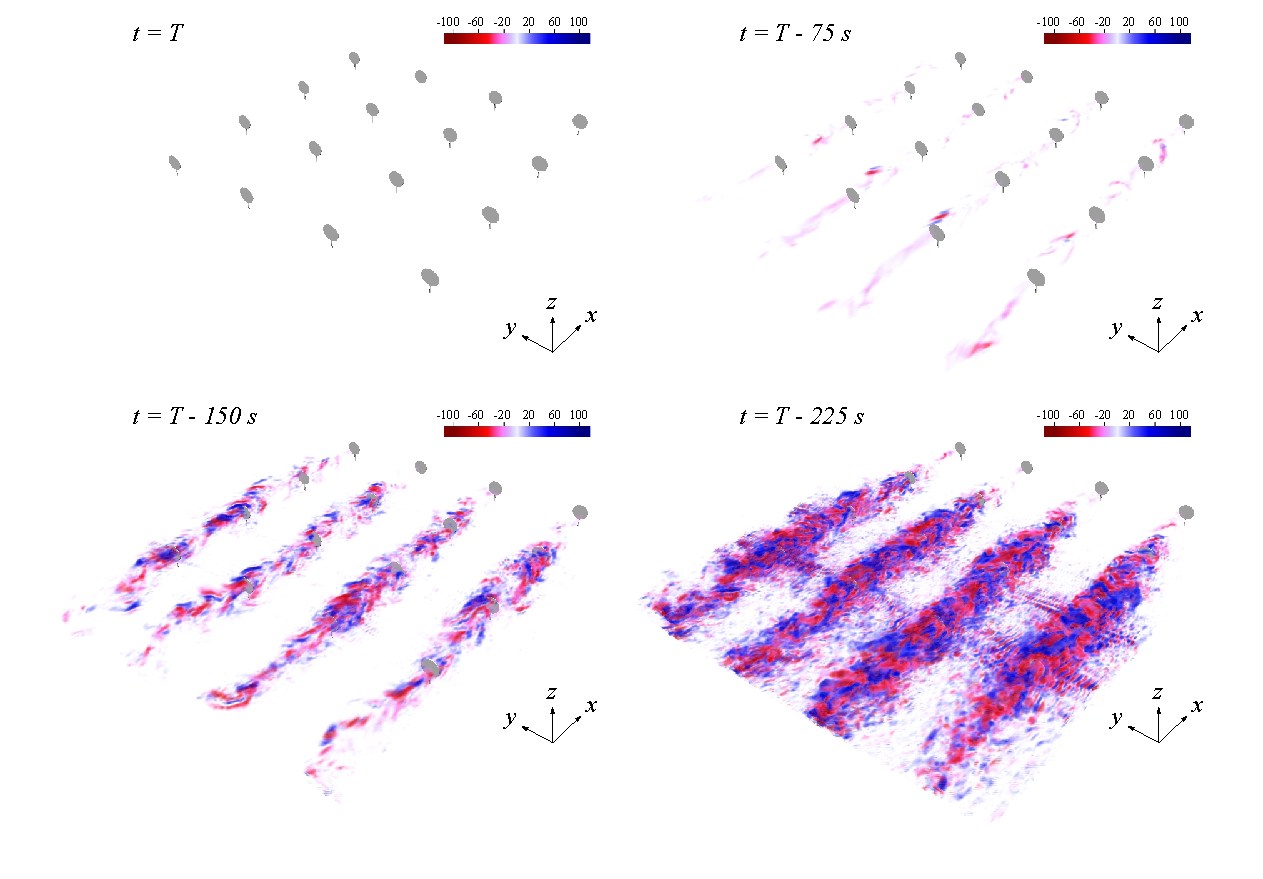
\includegraphics[width=\textwidth]{chapters/optimal_control_problem/adjoint_3D.eps}
		\caption{Volume rendering of streamwise adjoint velocity component $\xi_x$ at different time instances for an optimal control problem with time horizon $T$. \label{fig:adjoint_3D}}
	\end{figure}


	\subsection{Gradient of the reduced cost functional}\label{sec:problem_gradient2}
	Equation \eqref{eq:adjoint_grad_concept} illustrates how the gradient of the reduced cost functional can be expressed without explicit reference to the state variation $\delta \bs{q}$. Further, the definition of the cost functional in \eqref{eq:costfunction} shows that $\partial \J / \partial \bs{\varphi} = 0$. The gradient can hence be evaluated as $\nabla \Jtilde = \big[ \partial \bs{B} / \partial \bs{\varphi}  \big]^* \bs{q}^*$, resulting in
	\begin{equation}\label{eq:problem_gradient}
		\nabla \Jtilde \equiv 
		\begin{bmatrix*}[l]
			\partial \Jtilde / \partial \bs{C}_T' \\
			\partial \Jtilde / \partial \bs{\omega} 
		\end{bmatrix*} = 
		\begin{bmatrix}
			- \bs{\sigma}\\
			- \bs{\eta}
		\end{bmatrix}
	\end{equation}
	The derivation is straightforward and elaborated in Appendix~\ref{ch:app_adj_der}.
	
	\subsection{Verification of the adjoint gradient}\label{sec:problem_verification}
	The current section aims to verify the continuous adjoint method applied in this manuscript through comparison with a finite-difference approximation of the cost functional gradient. Since the accuracy of the continuous adjoint method is dependent on the spatiotemporal resolution with which the equations are discretized, the test is performed on a case with resolution similar to the cases defined in the following chapters. To limit computational cost, we consider a domain of reduced size with only 2 aligned turbines. The simulation domain of $2.5 \times 0.6 \times 1$ km$^3$ is discretized on a grid of $96 \times 48 \times 144$, resulting in a grid resolution of $26 \times 12.5 \times 6.9$ m$^3$. 
	
	The finite difference method approximates the G\^ateaux derivative in a direction $\delta \bs{\varphi}$ defined in Equation \eqref{eq:gateauxder} as
	\begin{equation}\label{eq:finitediff_grad}
		\innerproduct{\nabla \Jtilde}{\delta \bs{\varphi}} \approx \frac{\Jtilde(\bs{\varphi} + \alpha \delta \bs{\varphi}) - \Jtilde(\bs{\varphi})}{\alpha},
	\end{equation}
	where $\alpha$ is sufficiently small yet large enough to avoid round-off errors due to finite-precision floating-point arithmetic. In the current work, $\alpha$ is chosen such that control perturbations are fives orders of magnitude smaller than baseline controls. As indicated earlier, approximating the full gradient $\nabla \Jtilde$ would require evaluating Equation \eqref{eq:finitediff_grad} for as many linearly independent directions $\delta \bs{\varphi}$ as there are dimensions in $\bs{\varphi}$. Here, we only evaluate a limited amount of gradient components, by choosing a set of pointwise perturbations $\delta \varphi_i(t^*) =\diracdelta(t-t^*)$ to the baseline controls of each of the turbines $i$ at different times $t^*$. 
	
	Figure~\ref{fig:forwardfield_adjointfield} illustrates snapshots of both the forward and adjoint solutions at hub height. From Figure~\ref{fig:forwardfield_adjointfield}b it can be seen that the adjoint field starts out as streamtubes from the turbines indicating where immediate changes in the cost function originate, and transitions to a chaotic field after some upstream distance. 
	
	\begin{figure}[t]
		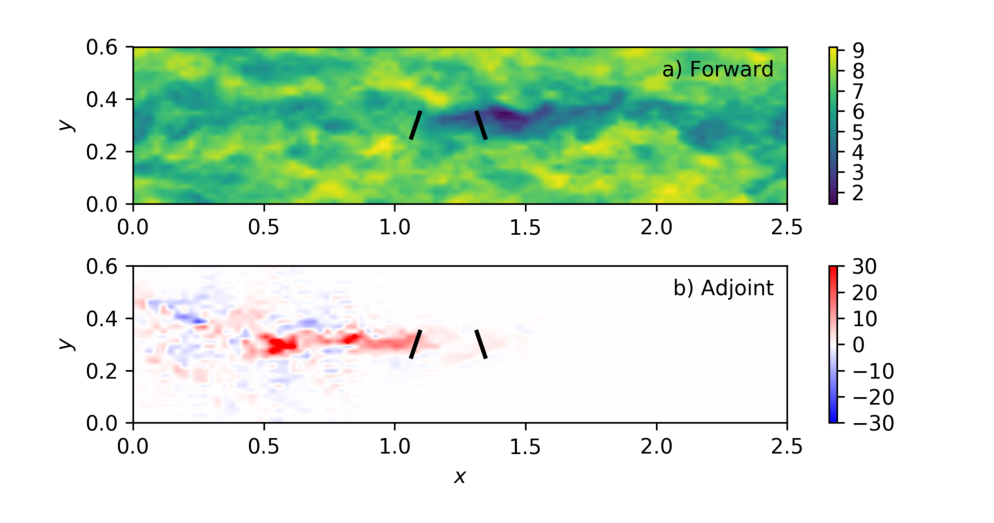
\includegraphics[width=\textwidth]{chapters/optimal_control_problem/forward_v_adjoint.eps}
	\caption[Solution fields for adjoint gradient verification test case at $t=150$ s.]{Solution fields for adjoint gradient verification test case at $t=150$ s. \emph{a)} Forward field $\tilde{u}_x$. \emph{b)} Adjoint field $\xi_x$. \label{fig:forwardfield_adjointfield}}
	\end{figure}

	Figure~\ref{fig:gradient_verification} illustrates the baseline controls $\bs{\varphi}$ around which the linearization is performed, as well as the adjoint gradient (full lines) compared to the finite difference gradient component approximations described above (dots). It can be seen from the figure that, throughout the entire time horizon, the gradient approximations match well. The overall relative error between both is about 2$\%$. Note that, although this error could be further reduced through grid refinement, we will show later that the current gradient accuracy is adequate for the optimizations considered in this work.
	
	\begin{figure}[b]
		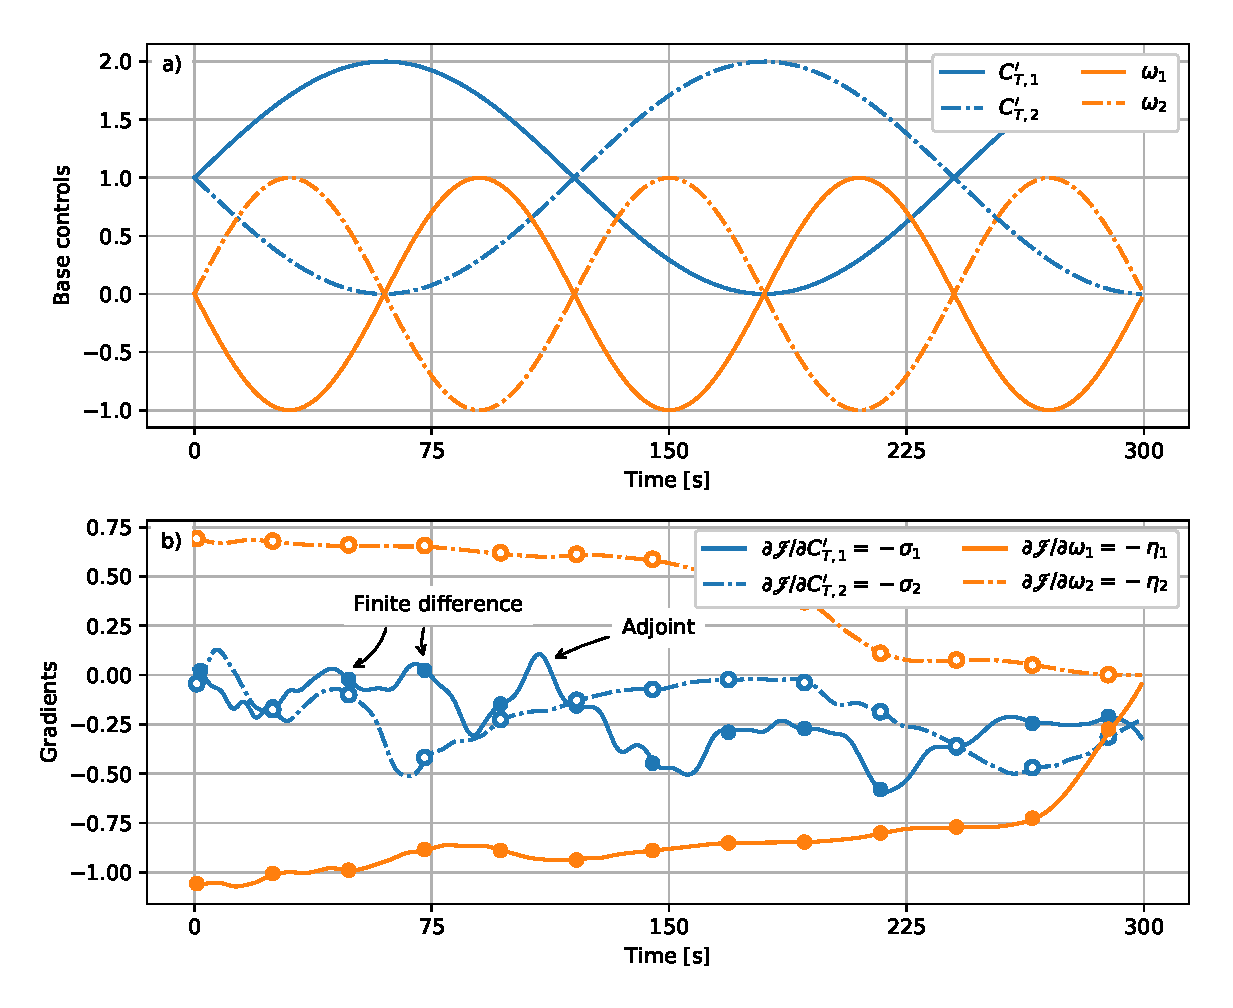
\includegraphics[width=\textwidth]{chapters/optimal_control_problem/gradient_verification.eps}
		\caption[Adjoint gradient verification case.]{Adjoint gradient verification case. \emph{a)} Baseline controls around which linearization is performed. \emph{b)} Cost functional gradient. Full lines: adjoint, dots: finite-difference. \label{fig:gradient_verification}}
	\end{figure}

\section{Summary}\label{sec:opt_prob_summ}
This chapter elaborated on the problem formulation and optimization methodology for the coordinated wind-farm control purposes considered in this work. Firstly, the receding horizon approach was elucidated, and a distinction of the current work with the conventional model-predictive control studies found in literature was made. Thereafter, the wind-farm control goal was mathematically formulated as a PDE-constrained optimization problem. Next, the use of a gradient-based quasi--Newton L--BFGS--B algorithm was justified based on an improved convergence behavior of the cost functional with respect to the total amount of PDE evaluations throughout the optimization process. The continuous adjoint approach for efficient gradient evaluation was introduced, and the adjoint gradient was verified through a comparative study with a finite difference gradient for a two-turbine test case. 

The following chapters focus on the application of the methodology introduced here. The considered cases differ mainly through the specification of the box constraints in Equations \eqref{eq:boxct_constraint} - \eqref{eq:boxomega_constraint}. Chapter~\ref{ch:opt_induction} focuses exclusively on optimal axial induction control (i.e. $\omega_{\text{max}} = 0$) by dynamically varying $C_T'$ for a set of wind farms with various layouts consisting of 72 turbines, and Chapter~\ref{ch:opt_analysis} further analyses resulting optimal control dynamics towards the design of practical induction controllers for wind farms. Chapter~\ref{ch:opt_yaw} further includes yaw control (i.e. $\omega_{\text{max}} \neq 0$) for a wind farm of reduced size with 16 turbines. 


%%%%%%%%%%%%%%%%%%%%%%%%%%%%%%%%%%%%%%%%%%%%%%%%%%
% Keep the following \cleardoublepage at the end of this file, 
% otherwise \includeonly includes empty pages.
\cleardoublepage
